% This is samplepaper.tex, a sample chapter demonstrating the
% LLNCS macro package for Springer Computer Science proceedings;
% Version 2.20 of 2017/10/04
%
\documentclass[runningheads]{llncs}
%
\usepackage{graphicx}

%custom packages
\usepackage{amsmath}
\usepackage{amssymb}
\usepackage{cite}
\usepackage{subfig}
\usepackage[labelfont=bf,labelsep=period]{caption}

\usepackage[utf8]{inputenc}
\inputencoding{utf8}
\usepackage[english, russian]{babel}

\DeclareMathOperator*{\argmax}{arg\,max}
\DeclareMathOperator*{\argmin}{arg\,min}
\DeclareMathOperator{\sign}{sign}
% Used for displaying a sample figure. If possible, figure files should
% be included in EPS format.
%
% If you use the hyperref package, please uncomment the following line
% to display URLs in blue roman font according to Springer's eBook style:
% \renewcommand\UrlFont{\color{blue}\rmfamily}

\begin{document}
%
\title{Parallel global optimization algorithm for obtaining uniform convergence when simultaneously solving a set of global optimization problems\thanks{This study was supported by the Russian Science Foundation, project No.\,16-11-10150.}}
%
%\titlerunning{Abbreviated paper title}
% If the paper title is too long for the running head, you can set
% an abbreviated paper title here
%
\author{Vladislav Sovrasov\and
Konstantin Barkalov
}
%
\authorrunning{V. Sovrasov et al.}
% First names are abbreviated in the running head.
% If there are more than two authors, 'et al.' is used.
%
\institute{Lobachevsky State University of Nizhny Novgorod, Nizhny Novgorod, Russia
\email{sovrasov.vladislav@itmm.unn.ru},
\email{konstantin.barkalov@itmm.unn.ru}
}
%
\maketitle              % typeset the header of the contribution
%
\begin{abstract}
    В данной работе рассматривается построение параллельной версии алгоритма глобальной оптимизации, решающего одновременно множество задач с нелинейными ограничениями и получающего при этом равномерные оценки решений на этом множестве. Последнее свойство позволяет наиболее оптимально распределять вычислительные ресурсы, т. к. в процессе работы алгоритма погрешности численного решения во всех задачах убывают примерно с одинаковой скоростью. Алгоритм присваивает приоритет каждой задаче и на каждой итерации производит вычисления целевых функций в нескольких задачах параллельно. При окончании работы метода в произвольный момент времени во всех задачах из решаемой серии будут получены решения сходного качества. Серии из нескольких задач возникают, если задача глобальной оптимизации имеет дискретный параметр или, например, при решении задачи многокритериальной оптимизации методом свертки критериев. Рассматриваемый алгоритм использует отображения типа кривой Пеано для редукции многомерных задач оптимизации к одномерным. Эффективность реализованного алгоритма протестирована на наборах искусственно сгенерированных задач глобальной оптимизации, а также при решении серии задач, полученной в результате скаляризации задачи многокритериальной оптимизации. Также экспериментально подтверждена равномерная сходимость метода.

\keywords{Global optimization \and Uniform convergence \and Derivative-free optimization \and Parallel computations.}
\end{abstract}
%
%
%

\section{Введение}
\label{sec-intro}
Нелинейная глобальная оптимизация невыпуклых функций традиционно считается одной из самых трудных
задач математического программирования. Отыскание глобального минимума функции от нескольких переменных
зачастую оказывается сложнее, чем локальная оптимизация в тысячемерном пространстве. Для последней может оказаться достаточно
применения простейшего метода градиентного спуска, в то время как чтобы \textit{гарантированно} отыскать глобальный оптимум методам
оптимизации приходится накапливать информацию о поведении целевой функции во всей области поиска \cite{Jones2009,Paulavicius2011,Evtushenko2013,Strongin2000}. Решение серии таких задач при ограниченных вычислительных
ресурсах является еще более сложной задачей: помимо поиска глобального экстремума необходимо
распределять вычислительные ресурсы так, чтобы сразу во всех решаемых задачах положение глобального
экстремума было оценено примерно с одинаковым качеством. Обычно серию из \(q\) задач решают либо последовательно, либо
параллельно порциями по \(p\ll q\) задач, где \(p\) --- количество параллельных вычислительных устройств.
Такой подход ведет к тому, что в каждый момент времени до окончания вычислений
остаются задачи, в которых оценка глобального оптимума не получена вообще, в то время, как в задачах из начала
списка оптимум может быть оценен даже с избыточной точностью.

В данной работе рассматривается обобщение ранее разработанного в ННГУ им. Н. И. Лобачевского
параллельного метода глобальной оптимизации для одновременного решения множества задач \cite{BarkalovStrongin2018} на
случай задач с нелинейными ограничениями. Для учета ограничений используется индексная схема \cite{Strongin2000},
позволяющая работать с частично вычислимыми целевым функциями и обладающая экономичностью,
сравнимой с другими подходами \cite{BarkalovLebedev2017}. Эффективность реализованного
алгоритма показана на примере решения множеств задач, сгенерированных специализированным
механизмом, порождающим наборы задач заданной размерности с заданным количеством нелинейных ограничений \cite{GergelBarkalov2019}.
Кроме искусственно сгенерированных задач, рассматриваемый метод протестирован также
на множестве задач, возникающем при решении задачи многокритериальной оптимизации
с нелинейными ограничениями методом свертки критериев \cite{Ehrgott2005}.

Статья имеет следующую структуру. В разделе \ref{sec:problem} рассмотрена
постановка решаемой задачи, далее в разделе \ref{sec:method} приведено описание
параллельного метода оптимизациии. Результаты численных экспериментов, подтверждающие
эффективность рассматриваемого метода приводятся в разделе \ref{sec:exps}.
В заключении приводится краткая сводка результатов, полученных в ходе работы, и
указаны направления дальнейших усилий по улучшению программной реализации рассмотренного метода.


\section{Постановка задачи глобальной оптимизации}
\label{sec:problem}
В рамках данной работы будем рассматривать следующую постановку задачи глобальной
оптимизации: найти глобальный минимум \(N\)-мерной функции \(\varphi(y)\) в гиперинтервале
\(D=\{y\in \mathbf{R}^N:a_i\leqslant x_i\leqslant{b_i}, 1\leqslant{i}\leqslant{N}\}\).
Для построения оценки глобального минимума по конечному количеству вычислений
значения функции требуется, чтобы скорость изменения \(\varphi(y)\) в \(D\) была ограничена.
В качестве такого ограничения как правило принимается условие Липшица.
\begin{equation}
\label{eq:task}
\varphi(y^*)=\min\{\varphi(y):y\in D\}
\end{equation}
\begin{displaymath}
\label{lip}
|\varphi(y_1)-\varphi(y_2)|\leqslant L\Vert y_1-y_2\Vert,y_1,y_2\in D,0<L<\infty
\end{displaymath}

Существуют различные методы, решающие рассмотренную многомерную задачу напрямую \cite{SergeyevKvasov2017, Jones2009},
а также эффективные методы решения одномерных задач \cite{Norkin1992, Strongin2000}. В данной работе рассматривается одномерный метод,
который применяется совместно со схемой редукции размерности.
Классической схемой редукции размерности исходной задачи для алгоритмов глобальной оптимизации является
использование разверток --- кривых, заполняющих пространство \cite{Sergeyev2013}.
\begin{equation}
\label{cube}
\lbrace y\in \mathbf{R}^N:-2^{-1}\leqslant y_i\leqslant 2^{-1},1\leqslant i\leqslant N\rbrace=\{y(x):0\leqslant x\leqslant 1\}
\end{equation}

Отображение вида (\ref{cube}) позволяет свести задачу в многомерном пространстве к решению
одномерной ценой ухудшения ее свойств. В частности, одномерная функция \(\varphi(y(x))\)
является не Липшицевой, а Гёльдеровой:
\begin{displaymath}
\label{holder}
|\varphi(y(x_1))-\varphi(y(x_2))|\leqslant H{|x_1-x_2|}^{\frac{1}{N}},x_1,x_2\in[0;1],
\end{displaymath}
где константа Гельдера \(H\) связана с константой Липшица \(L\) соотношением
\begin{displaymath}
H=4Ld\sqrt{N},d=\max\{b_i-a_i:1\leqslant i\leqslant N\}.
\end{displaymath}

Область \(D\) также может быть задана с помощью функциональных ограничений, что
значительно усложняет задачу.
Постановка задачи глобальной оптимизации в этом случае будет иметь следующий вид:
\begin{equation}
  \label{eq:constrained_problem}
  \varphi(y^*)=\min\{\varphi(y):g_j(y)\leqslant 0, 1\leqslant j\leqslant m\}
\end{equation}
Обозначим \(g_{m+1}(y)=\varphi(y)\). Далее будем предполагать, что все функции \(g_k(y),1\leqslant k \leqslant m+1\)
удовлетворяют условию Липшица в некотором гиперинтервале, включающем \(D\).

Далее будем интересоваться решением серии из \(q\) задач вида (\ref{eq:constrained_problem}):
\begin{equation}
  \label{eq:many_problems}
  \min\left\{\varphi_1(y), y\in D_1 \right\}, \min\left\{\varphi_2(y), y\in D_2\right\},..., \min\left\{\varphi_q(y), y\in D_q\right\}.
\end{equation}

\section{Описание метода глобальной оптимизации}
\label{sec:method}

Принимая во внимание схему редукции размерности (\ref{cube}), будем при описании метода считать, что
требуется найти глобальный минимум функции \(\varphi(x), x\in[0;1]\),
удовлетворяющей условию Гёльдера, при ограничениях \(g_j(x)\), также
удовлетворяющих этому условию на интервале \([0;1]\).

Рассматриваемый индексный алгоритм глобального поиска (ИАГП) для решения
одномерной задачи (\ref{eq:constrained_problem}) предполагает построение последовательности
точек \(x_k\), в которых вычисляются значения минимизируемой функции или ограничений \(z_k = g_s(x_k)\).
Для учета последних используется индексная схема \cite{Strongin2000}. Пусть \(Q_0=[0;1]\). Ограничение, имеющее номер
 \(j\), выполняется во всех точках области
\begin{displaymath}
  Q_j=\left\{x\in [0;1]:g_j(x)\leq 0\right\},
\end{displaymath}
которая называется допустимой для этого ограничения. При этом допустимая область \(D\)
исходной задачи определяется равенством: \(D=\cap _{j=0}^{m}Q_{j}\).
Испытание в точке \(x\in [0;1]\) состоит в последовательном вычислении значений
величин \(g_{1}(x),...,g_{\nu }(x)\), где значение индекса \(\nu\) определяется условиями:
\(x\in Q_{j},0\leqslant j<\nu ,x\notin Q_{\nu }\). Выявление первого нарушенного ограничения
прерывает испытание в точке \(x\). В случае, когда точка \(x\)  допустима, т. е.
\(x\in D\) испытание включает в себя вычисление всех функций задачи. При этом значение
индекса принимается равным величине \(\nu =m+1\). Пара \(\nu =\nu (x),z=g_{\nu }(x)\),
где индекс \(\nu\) лежит в границах \(1\leqslant \nu \leqslant m+1\), называется результатом
испытания в точке \(x\).

Такой подход к проведению испытаний позволяет свести исходную задачу с функциональными
ограничениями к безусловной задаче минимизации разрывной функции:

\begin{displaymath}
  \begin{array}{lr}
    \psi (x^{*})=\min_{x\in [0;1]}\psi (x), \\
    \psi (x)={\begin{cases}g_{\nu }(x)/H_{\nu }&\nu <M\\(g_{M}(x)-g_{M}^{*})/H_{M}&\nu =M\end{cases}}
  \end{array}
\end{displaymath}

Здесь \(M=\max_{}^{}\left\{\nu (x):x\in [0;1]\right\}\), а \(g_{M}^{*}=\min _{}^{}\left\{g_{M}(x):x\in \cap _{i=0}^{M-1}Q_{i}\right\}\).
В силу определения числа \(M\), задача отыскания \(g_{M}^{*}\)
всегда имеет решение, а если \(M=m+1\), то \(g_{M}^{*}=\varphi(x^{*})\).
Дуги функции \(\psi (x)\) гельдеровы на множествах \(\cap _{i=0}^{j}Q_{i},0\leq j\leq M-1\)
с константой 1, а сама \(\psi (x)\) может иметь разрывы первого рода на границах этих множеств.
Несмотря на то, что значения констант Гёльдера \(H_k\) и величина \(g_{M}^{*}\) заранее неизвестны,
они могут быть оценены в процессе решения задачи.

Множество троек \(\{(x_k,\nu_k,z_k)\}, 1\leqslant k\leqslant n\) составляет поисковую информацию,
накопленную методом после проведения \(n\) шагов.

На первой итерации метода испытание проводится в произвольной внутренней точке \(x_1\)
интервала \([0;1]\). Индексы точек 0 и 1 считаются нулевыми, значения \(z\) в
них не определены. Пусть выполнено \(k\geqslant 1\) итераций метода,
в процессе которых были проведены испытания в \(k\) точках \(x_i, 1\leqslant i\leqslant k\).
Тогда точка \(x^{k+1}\) поисковых испытаний следующей \((k+1)\)-ой
итерации определяются в соответствии с правилами:

Шаг 1. Перенумеровать точки множества \(X_k=\{x^1,\dotsc,x^k\}\cup\{0\}\cup\{1\}\),
которое включает в себя граничные точки интервала \([0;1]\), а также точки предшествующих
испытаний, нижними индексами в порядке увеличения значений координаты, т.е.
\begin{displaymath}
0=x_0<x_1<\dotsc<x_{k+1}=1
\end{displaymath}
и сопоставить им значения \(z_{i}=g_{\nu }(x_{i}),\nu =\nu (x_{i}),i={\overline {1,k}}\).

Шаг 2. Для каждого целого числа \(\nu ,1\leqslant \nu \leqslant m+1\) определить соответствующее
ему множество \(I_{\nu }\) нижних индексов точек, в которых вычислялись значения
функций \(g_{\nu }(x)\):
\begin{displaymath}
  I_{\nu }=\{i:\nu (x_{i})=\nu ,1\leqslant i\leqslant k\},1\leq \nu \leqslant m+1,
\end{displaymath}
определить максимальное значение индекса \(M=\max\{\nu (x_{i}),1\leq i\leq k\}\).

Шаг 3. Вычислить текущие оценки для неизвестных констант Гёльдера:
\begin{equation}
  \label{step2}
  \mu _{\nu }=\max\{\frac{|g_{\nu }(x_{i})-g_{\nu }(x_{j})|}{(x_{i}-x_{j})^{\frac{1}{N}}}:i,j\in I_{\nu },i>j\}.
\end{equation}
Если множество \(I_{\nu }\) содержит менее двух элементов или если значение \(\mu _{\nu }\)
оказывается равным нулю, то принять \(\mu _{\nu }=1\).

Шаг 4. Для всех непустых множеств \(I_{\nu },\nu ={\overline {1,M}}\) вычислить оценки
\begin{displaymath}
  z_{\nu }^{*}={\begin{cases}\min\{g_{\nu }(x_{i}):x_{i}\in I_{\nu }\}&\nu =M\\-\varepsilon _{\nu }&\nu <M\end{cases}},
\end{displaymath}
где вектор с неотрицательными координатами \(\varepsilon _{R}=(\varepsilon _{1},..,\varepsilon _{m})\) называется вектором резервов.

Шаг 5. Для каждого интервала \((x_{i-1};x_{i}),1\leqslant i\leqslant k\) вычислить характеристику
\begin{equation}
  \label{step3_1}
  R(i)={\begin{cases}\Delta _{i}+{\frac {(z_{i}-z_{i-1})^{2}}{(r_{\nu }\mu _{\nu })^{2}\Delta _{i}}}-2{\frac {z_{i}+z_{i-1}-2z_{\nu }^{*}}{r_{\nu }\mu _{\nu }}}&\nu =\nu (x_{i})=\nu (x_{i-1})\\2\Delta _{i}-4{\frac {z_{i-1}-z_{\nu }^{*}}{r_{\nu }\mu _{\nu }}}&\nu =\nu (x_{i-1})>\nu (x_{i})\\2\Delta _{i}-4{\frac {z_{i}-z_{\nu }^{*}}{r_{\nu }\mu _{\nu }}}&\nu =\nu (x_{i})>\nu (x_{i-1})\end{cases}}
\end{equation}
где \(\Delta _{i}=(x_{i}-x_{i-1})^{\frac{1}{N}}\). Величины \(r_{\nu }>1,\nu ={\overline {1,m}}\)
являются параметрами алгоритма. От них зависят произведения \(r_{\nu }\mu _{\nu }\),
используемые при вычислении характеристик в качестве оценок неизвестных констант Гёльдера.

Шаг 6. Выбрать наибольшую характеристику:
\begin{equation}
\label{step4}
t=\argmax_{1\leqslant i \leqslant k+1}R(i)
\end{equation}

Шаг 7. Провести очередное испытание в середине интервала \((x_{t-1};x_{t})\),
если индексы его концевых точек не совпадают: \(x^{k+1}={\frac {1}{2}}(x_{t}+x_{t-1})\).
В противном случае провести испытание в точке
\begin{displaymath}
  x^{k+1}={\frac {1}{2}}(x_{t}+x_{t-1})-\operatorname {sgn}(z_{t}-z_{t-1}){\frac {|z_{t}-z_{t-1}|^{n}}{2r_{\nu }\mu _{\nu }^{n}}},\nu =\nu (x_{t})=\nu (x_{t-1}),
\end{displaymath}
а затем увеличить \(k\) на 1.

Алгоритм прекращает работу, если выполняется условие \(\Delta_{t}\leqslant \varepsilon\),
где \(\varepsilon>0\) есть заданная точность. В качестве оценки глобально-оптимального решения выбираются значения
\begin{equation}
\varphi_k^*=\min_{1\leqslant i \leqslant k}\varphi(x_i), x_k^*=\argmin_{1\leqslant i \leqslant k}\varphi(x_i)
\end{equation}

Далее следуя подходу, описанному в \cite{BarkalovStrongin2018}, для решения серии задач (\ref{eq:many_problems}) будем
использовать \(q\) синхронно работающих копий ИАГП с тем лишь отличием, что на шаге 6 при выборе
интервала с наилучшей характеристикой, выбор будет осуществляться из всех интервалов, которые
породили на данный момент \(q\) копий ИАГП. Если наибольшая характеристика соответствует
задаче \(i\), то выполняется шаг 7 в копии метода с номером \(i\), а остальные копии метода простаивают.
Таким образом, на каждой итерации испытание проводится в задаче, наиболее перспективной с точки зрения
характеристик (\ref{step3_1}), что позволяет динамически распределять ресурсы метода между задачами.

В \cite{BarkalovStrongin2018} приведена теория сходимости такого подхода на случай решения задач без ограничений.
При наличии ограничений характеристики интервалов, на концах которых нарушено разное количество ограничений,
вычисляются в соответствии с нижними строчками из (\ref{step3_1}). Нетрудно заметить, что и в этом случае
величины характеристик нормированы, а в случае точных оценок \(z_{\nu }^{*}\) и \(\mu _{\nu }\) их
масштаб не зависит от целевой функции и ограничений конкретной задачи. Таким образом, рассуждения
из \cite{BarkalovStrongin2018} можно провести и в случае использования индексной схемы.

Параллельная модификация метода не отличается от рассматриваемой в \cite{BarkalovStrongin2018}
и заключается в выборе \(p\) интервалов на шаге 6 и выполнения \(p\) испытаний параллельно
на следующем шаге. При этом все ресурсы метода в рамках итерации могут быть направлены как на одну, так и
на \(l\leqslant p\) задач одновременно (в зависимости от того, какой из задач принадлежат выбранные методам интервалы).

\section{Результаты численных экспериментов}
\label{sec:exps}

Использование сгенерированных некоторыми случайными механизмами
наборов тестовых задач с известными решениями является одним из общепринятых подходов
к сравнению алгоритмов оптимизации \cite{Beiranvand2017}. В данной работе
будем использовать два генератора тестовых задач, порождающих задачи различной природы \cite{grishaginClass, Gaviano2003}.
Эти генераторы порождают задачи без нелинейных ограничений, поэтому в дополнение к ним использована
система GCGen\footnote{Исходный код системы доступен по ссылке https://github.com/UNN-ITMM-Software/GCGen} \cite{GergelBarkalov2019}, позволяющая генерировать задачи с ограничениями на основе произвольных нелинейных
функций.

Вместе с системой GCGen распространяются примеры ее использования и построения
наборов задач, каждая из которых состоит из целевой функции и двух ограничений,
порожденных генератором \(F_{GR}\) \cite{grishaginClass} или GKLS \cite{Gaviano2003}.

% Обозначим набор из 50 задач, полученных с помощью GCGen и первого генератора из \cite{grishaginClass} как \(F_{GR}^C\). Механизм построения функций \(F_{GR}\) не предусматривает контроля за размерностью (она равна 2) и количеством локальных оптимумов, однако известно, что порождаемые функции
% являются существенно многоэкстремальными.

Генератор GKLS \cite{Gaviano2003} позволяет получать функции заданной размерности и с заданным количеством экстремумов.
В сочетании с GCGen были порождены два множества по 100 задач размерности 2 и 3. Каждая из задач имеет два ограничения.
Также с целью демонстрации того, что свойства метода сохраняются при существенно разных свойствах задач
был сгенерирован смешанный класс, состоящий из 50 задач с двухмерными функциями GKLS и 50 задач с функциями \(F_{GR}\).
На рис. \ref{fig:isolines} представлены примеры линий уровня рассматриваемых задач. Допустимая область закрашена.

\begin{figure}[ht]
    \centering
    \subfloat[Решение внутри допустимой области]{
    {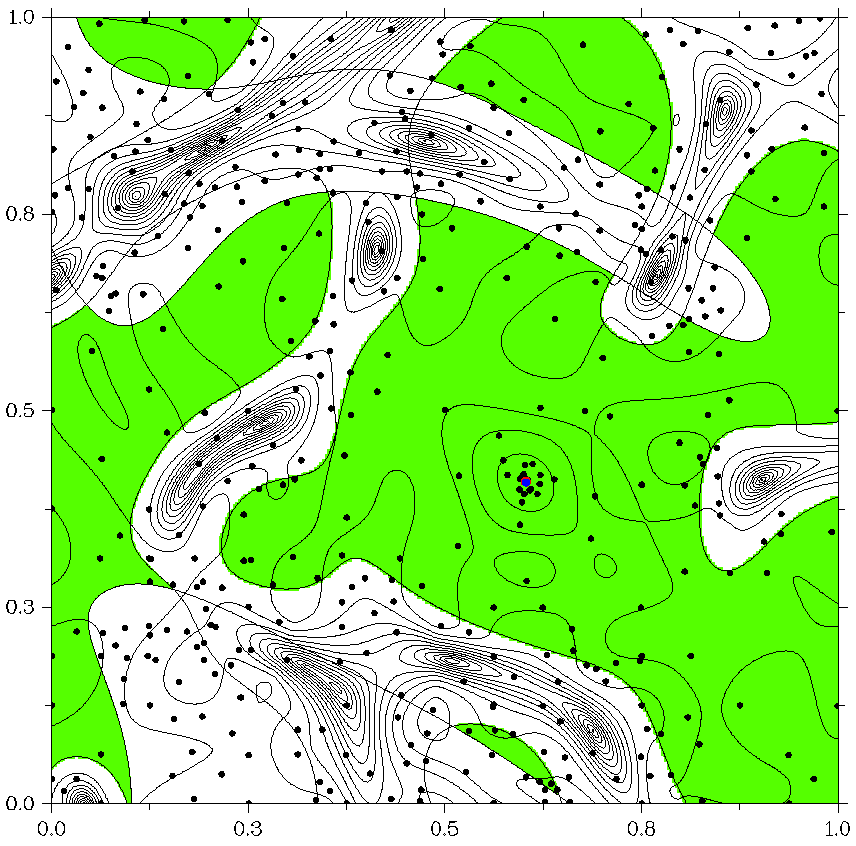
\includegraphics[width=.5\textwidth]{pic/2.png}}}
    \subfloat[Решение на границе допустимой области]{
    {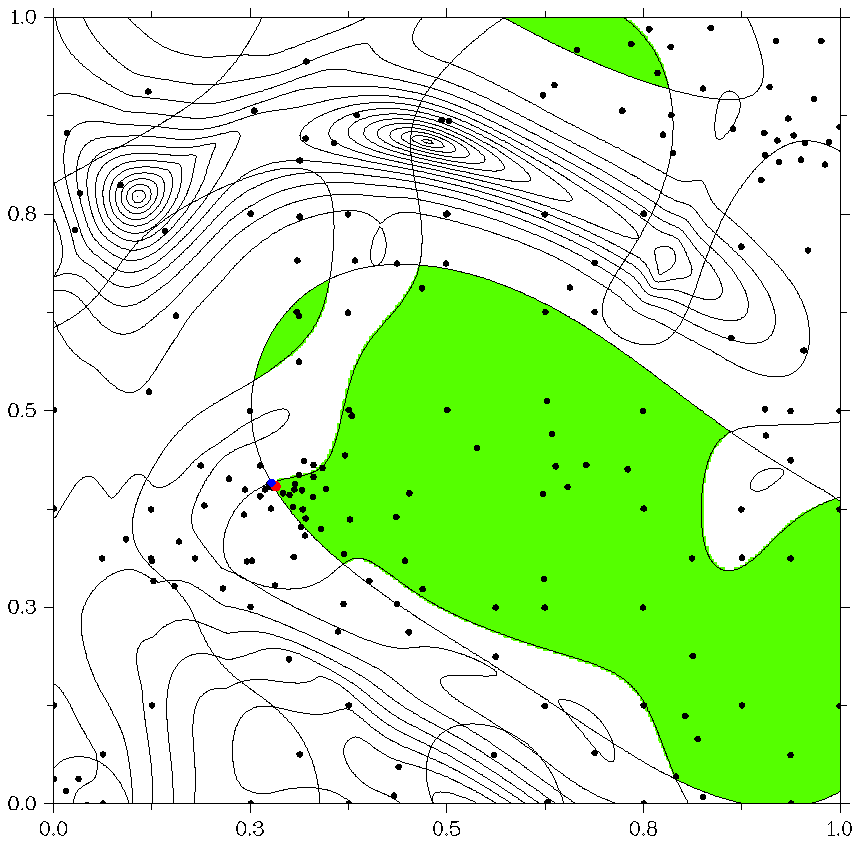
\includegraphics[width=.5\textwidth]{pic/4.png}}}
    \caption{Линии уровня и точки испытаний ИАГП в двух синтетических задачах}
    \label{fig:isolines}
\end{figure}

Будем считать, что тестовая задача решена, если метод оптимизации провел очередное испытание \(y^k\) в
\(\delta\)-окрестности глобального минимума \(y^*\), т.е. $\left\|y^k-
y^*\right\|\leqslant \delta = 0.01\left\|b-a\right\|$, где \(a\) и \(b\) --- левая и правая границы гиперкуба из (\ref{eq:task}).
Если указанное соотношение не выполнено до истечения лимита на количество испытаний, то задача считается нерешенной.

%В качестве характеристик метода оптимизации на каждом из классов будем рассматривать среднее число
%испытаний, затраченное для решения одной задачи, и количество решенных задач. Чем меньше число испытаний, тем быстрее метод сходится
%к решению, а значит и меньше обращается к потенциально трудоемкой процедуре вычислений целевой функции.
При оценке качества метода и его реализации кроме ускорения от распараллеливания и времени выполнения также будем принимать во внимание среднее максимальное расстояния (в смысле \(l_{\inf}\)-нормы) текущей оценки оптимума до его реального положения,
вычисленное на множестве задач (\ref{eq:many_problems}): \(D_{avg}\) и \(D_{max}\). Динамика этих величин в процессе оптимизации
показывает, насколько равномерно метод распределяет ресурсы между задачами.

Реализация параллельного метода была выполнена на языке C++ с использованием технологии OpenMP
для распареллеливания процесса проведения испытаний на общей памяти. Все вычислительные
эксперименты проведены на машине со следующей конфигурацией: Intel Core i7-7800X, 64GB RAM, Unubtu 16.04 ОS, GCC 5.5 compiler.

\subsection{Результаты решения сгенерированных задач}

Результаты решения тестовых задач последовательной и параллельной версией модифицированного ИАГП
для решения множества задач представлены в \ref{tab:speedup}. Для всех двухмерных классов задач параметр \(r=4.7\).
В случае трехмерных задач \(r=4.7,\: \varepsilon_\nu=0.1\).
Во всех экспериментах в целевые функции и ограничения была внесена дополнительная вычислительная нагрузка так,
чтобы время одного обращения к функции задачи было равно примерно 1мс.

Из таблицы видно, что ускорение по итерациям \(S_i\) растет линейно с увеличением числа потоков \(p\),
в то время, как ускорение по времени \(S_p\) увеличивается не так быстро, что говорит о неидеальной
реализации алгоритма. Увеличить реальное ускорение, верхней границей для которого является
\(S_i\), возможно путем оптимизации взаимодействий между копиями ИАГП и это планируется сделать в ходе будущей работы.

\begin{table}
  \centering
  \caption{Результаты экспериментов на наборах синтетических задач}
  \label{tab:speedup}
  \begin{tabular}{c|c|cccc}
    %\cline{1-8}\noalign{\smallskip}
    Класс задач & \textit{p} & Количество итераций & Время, с & \(S_i\) & \(S_t\)   \\
    %s\noalign{\smallskip} \cline{4-5} \cline{7-8}  \noalign{\smallskip}
    \hline
    GKLS \& \(F_{GR}\) based \
      & 1 & 51434 & 90.20 & -    & - \\
      & 2 & 25698 & 56.96 & 2.00 & 1.58 \\
      & 4 & 13015 & 36.67 & 3.95 & 2.46 \\
      & 6 & 8332  & 26.85 & 6.17 & 3.36 \\
    \hline
    GKLS based 2d \
      & 1 & 59066 & 97.53 & -    & - \\
      & 2 & 29060 & 60.56 & 2.04 & 1.61 \\
      & 4 & 14266 & 38.92 & 4.14 & 2.51 \\
      & 6 & 9436  & 29.53 & 6.26 & 3.30 \\
    \hline
    GKLS based 3d \
      & 1 & 782544 & 1117.55 & -    & - \\
      & 2 & 397565 & 752.92  & 1.97 & 1.48 \\
      & 4 & 208073 & 526.67  & 3.76 & 2.12 \\
      & 6 & 142089 & 445.45  & 5.50 & 2.51 \\
    \hline
  \end{tabular}
\end{table}

Для того, чтобы показать равномерную сходимость все тестовые задачи были также решены ИАГП
в режиме решения отдельных задач. На рис. \ref{fig:devs_mixed} указаны графики величин
средних и максимальных расстояний от реальных оптимумов до их текущих оценок при решении
серии из задач, порожденных двумя разными генераторами, по отдельности (сплошная кривая) и совместно (пунктирная кривая).
Не смотря на значительную разницу в структуре задач, модифицированный ИАГП
гораздо быстрее уменьшает как максимальное, так и среднее отклонение оценок от оптимумов.
Это говорит о наличии равномерной сходимости по всему множеству совместно решаемых задач.
При этом в случае последовательного решения задач величина \(D_{max}\) имеет наибольшее значение вплоть
до решения последней задачи.

\begin{figure}[ht]
    \centering
    \subfloat[\(D_{max}\)]{
    \label{fig:max_dev} {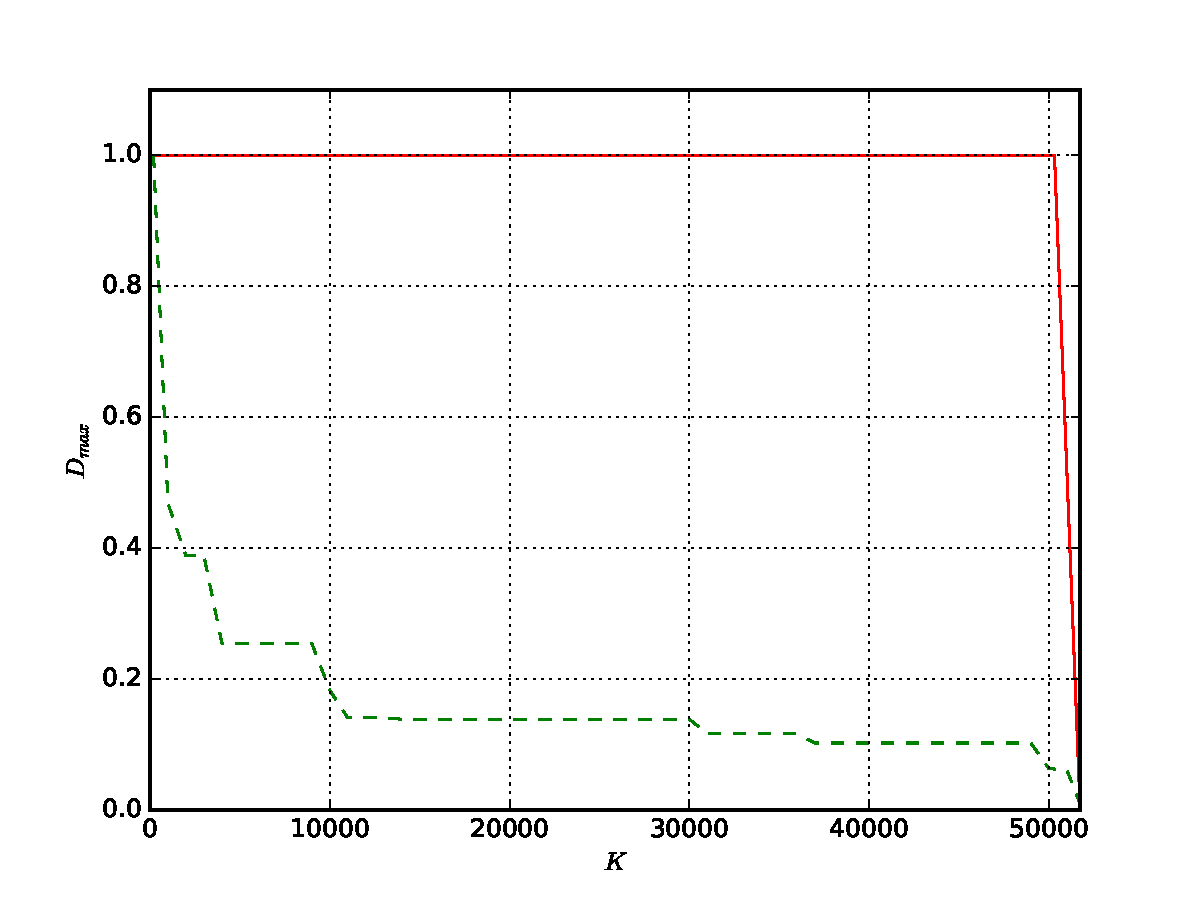
\includegraphics[width=.5\textwidth]{pic/mixed_2d_max.pdf}}}
    \subfloat[\(D_{avg}\)]{
    \label{fig:avg_dev} {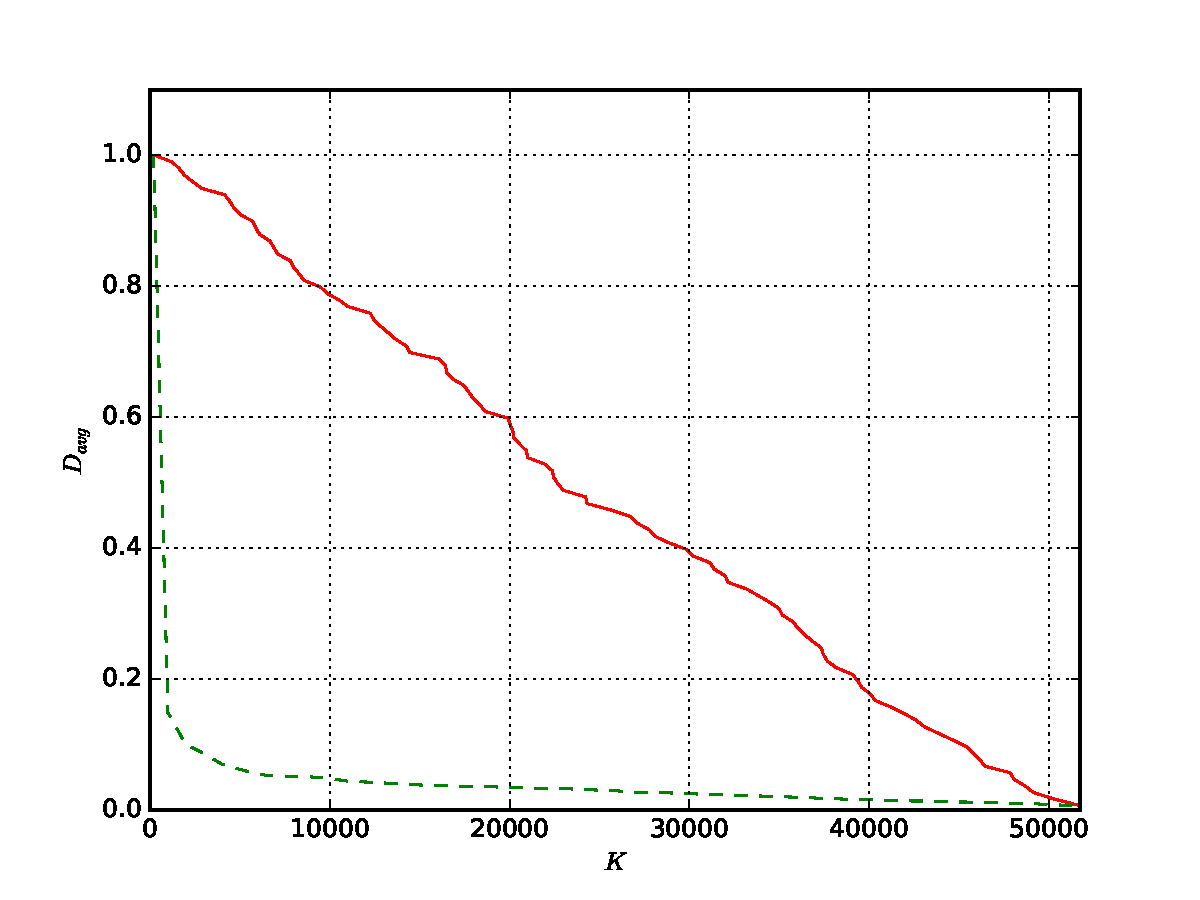
\includegraphics[width=.5\textwidth]{pic/mixed_2d_avg.pdf}}}
    \caption{Динамика величин \(D_{avg}\) и \(D_{max}\) в процессе решения множества двухмерных задач,
    порождённых двумя разными генераторами GKLS и \(F_{GR}\)}
    \label{fig:devs_mixed}
\end{figure}

\subsection{Пример решения многокритериальной задачи}

Для демонстрации эффективности подхода к балансировке нагрузки рассмотрим пример,
в котором множество задач вида (\ref{eq:many_problems}) порождено в результате скаляризации
многокритериальной задачи оптимизации с ограничениями.

Рассмотрим тестовую задачу, предложенную в \cite{BinhKorn1999}:
\begin{equation}
  \label{eq:mco_probem}
  \begin{array}{l}
      Minimize \left \{
      \begin{array}{l}
        f_1(y) = 4 y_1^2 + 4 y_2^2 \\
        f_2(y) = (y_1-5)^2 + (y_2-5)^2 \\
      \end{array}
      \right .
      y_1\in [-1;2],y_2\in [-2;1]
      \\s.t.
      \\
      \left \{
      \begin{array}{l}
        g_1(y) = (y_1 - 5)^2 + y_2^2 - 25 \leqslant 0 \\
        g_2(y) = -(y_1 - 8)^2 - (y_2 + 3)^2 + 7.7 \leqslant 0\\
      \end{array}
      \right .
  \end{array}
\end{equation}

Будем использовать свертку Гермейера для скаляризации задачи (\ref{eq:mco_probem}).
После свертки скалярная целевая функция имеет вид:
\begin{equation}
  \varphi(y,\lambda_1,\lambda_2)=\max\{\lambda_1 f_1(y), \lambda_2 f_2(y)\},
\end{equation}
где \(\lambda_1,\lambda_2\in[0,1],\: \lambda_1+\lambda_2=1\). Перебирая все возможные
коэффициенты свертки, можно найти все множество парето-оптимальных решений в
задаче (\ref{eq:mco_probem}). Для численного построения множества Парето выберем
100 наборов коэффициентов \((\lambda_1,\lambda_2)\) таких, что
\(\lambda_1^i=i h,\: \lambda_2^i=1-\lambda_1^i,\: h=10^{-2},i=\overline{1, 100}\).

В качестве ограничения на вычислительные ресурсы был выбран лимит в 2500 испытаний.
Множество вспомогательных скалярных задач решалось двумя способами:
\begin{itemize}
  \item каждая задача решается отдельно с помощью ИАГП с установленным лимитом в
  25 испытаний. Таким образом, вычислительные ресурсы равномерно распределены между задачами;
  \item все задачи решаются одновременно с помощью обобщенного ИАГП с установленным лимитом в
  2500 испытаний.
\end{itemize}
В обоих случаях параметр \(r=4\).

\begin{figure}[ht]
    \centering
    \subfloat[ИАГП, раздельное решение задач]{
    \label{fig:mco_pareto_1} {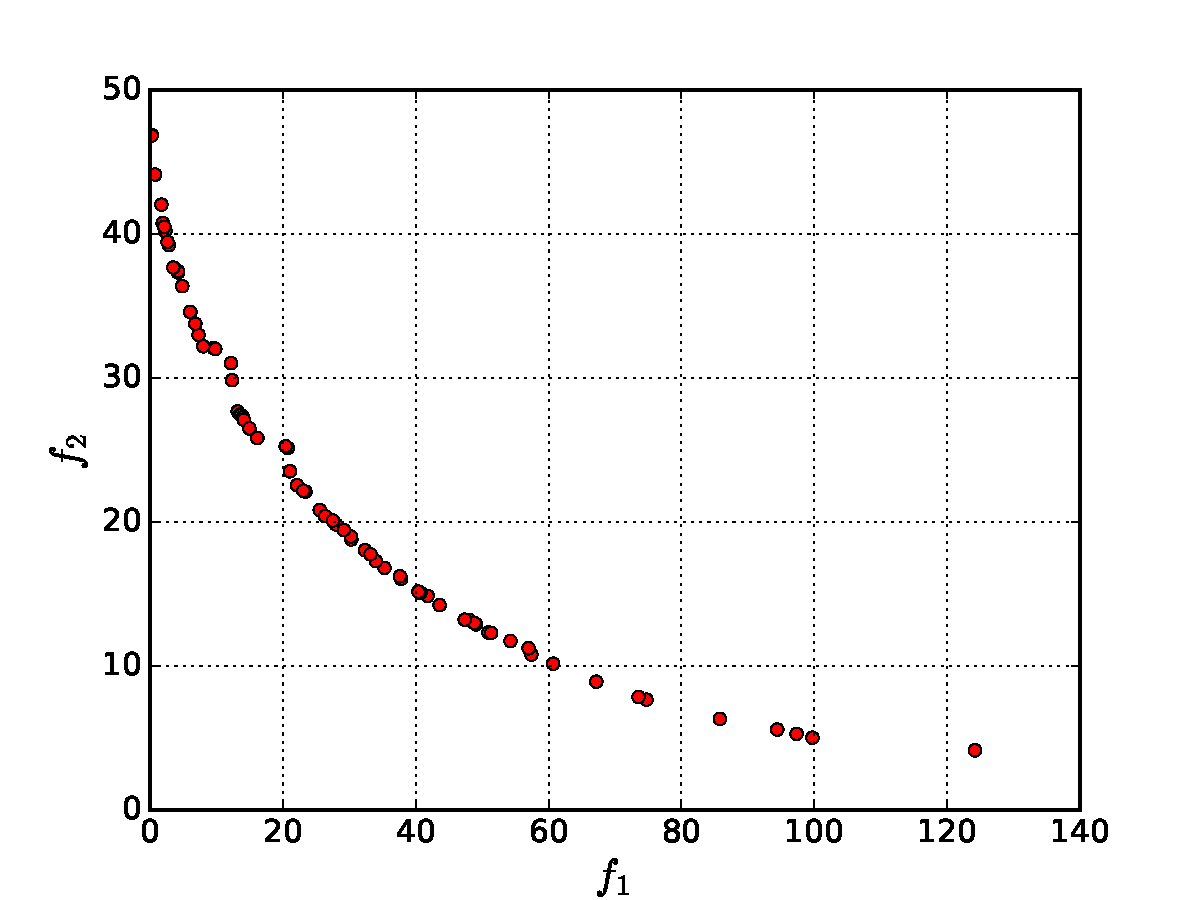
\includegraphics[width=.5\textwidth]{pic/single_mco.pdf}}}
    \subfloat[ИАГП для множества задач]{
    \label{fig:mco_pareto_2} {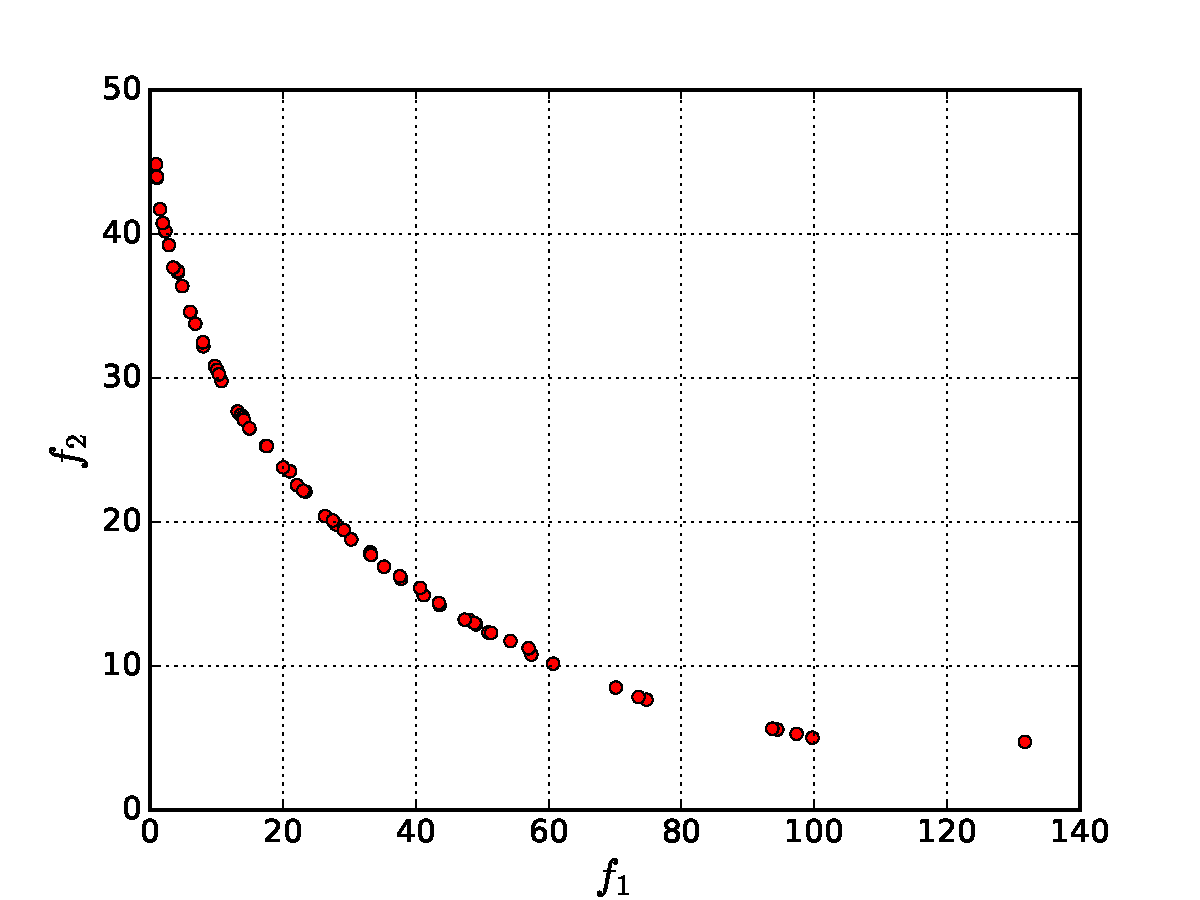
\includegraphics[width=.5\textwidth]{pic/multi_mco.pdf}}}
    \caption{Численные оценки множества Парето в задаче (\ref{eq:mco_probem}), полученные после 2500 испытаний}
    \label{fig:mco_pareto}
\end{figure}

На рис. \ref{fig:mco_pareto_1} и рис. \ref{fig:mco_pareto_2}
представлены графики решений, полученных каждым из методов.
Все графики качественно совпадают с указанным в \cite{BinhKorn1999} (авторы не предоставили другой
информации и решениях для сравнения). Видно, что на рис. \ref{fig:mco_pareto_1}
кривая Парето имеет вогнутости, что не соответствует решению, указанному в \cite{BinhKorn1999} и
означает нехватку ресурсов для решения некоторых из вспомогательных задач.
Для оценки качества решения также был вычислен показатель \(Spacing(SP)\) \cite{RiquelmeLucken2015},
характеризующий плотность точек аппроксимации множества Парето.
\begin{displaymath}
  SP(S)=\sqrt{\frac{1}{|S|-1} \sum_{i=1}^{|S|} (\overline{d}-d_i)^2},
  \:\overline{d}=mean\{d_i\},\:d_i=\min_{s_i,s_j\in S:s_i\ne s_j}||F(s_i)-F(s_j)||_1,\: F=(f_1,f_2)
\end{displaymath}
В случае отдельного решения задач \(SP_{single}=0.984\), а при решении задач методом с балансировкой нагрузки
\(SP_{multi}=0.749\), что говорит о более качественном приближении решения.

\section{Заключение}

В ходе работы была реализована поддержка нелинейных ограничений в алгоритме, решающeм
множество задач глобальной оптимизации. Проведены численные эксперименты, демонстрирующие
преимущество рассматриваемого подхода над решением задач по отдельности. Показана эффективность
совместного решения множества задач на примере решения многокритериальной задачи с
нелинейными ограничениями.

В ходе дальнейшей работы планируется улучшить текущую реализацию алгоритма,
сократив расходы на содержание поисковой информации для множества задач и тем самым улучшив
показатели параллельного ускорения по времени. Также планируется реализовать версию
рассматриваемого алгоритма, работающего на распределенной памяти по схеме, описанной в \cite{BarkalovLebedev2017_2}.

%
% ---- Bibliography ----
%
% BibTeX users should specify bibliography style 'splncs04'.
% References will then be sorted and formatted in the correct style.
%
% \bibliographystyle{splncs04}
% \bibliography{mybibliography}
%
\begin{thebibliography}{8}
\bibitem{ref_article1}
Author, F.: Article title. Journal \textbf{2}(5), 99--110 (2016)

\bibitem{ref_lncs1}
Author, F., Author, S.: Title of a proceedings paper. In: Editor,
F., Editor, S. (eds.) CONFERENCE 2016, LNCS, vol. 9999, pp. 1--13.
Springer, Heidelberg (2016). \doi{10.10007/1234567890}

\bibitem{ref_book1}
Author, F., Author, S., Author, T.: Book title. 2nd edn. Publisher,
Location (1999)

\bibitem{ref_proc1}
Author, A.-B.: Contribution title. In: 9th International Proceedings
on Proceedings, pp. 1--2. Publisher, Location (2010)

\bibitem{ref_url1}
LNCS Homepage, \url{http://www.springer.com/lncs}. Last accessed 4
Oct 2017
\end{thebibliography}
\end{document}
